\chapter{Specifikacija programske potpore}
		
	\section{Funkcionalni zahtjevi}
			

			

				

			
			
			\noindent \textbf{Dionici:}
			
			\begin{packed_enum}
				
				\item Administrator
				\item Moderator			
				\item Korisnici aplikacije
					\begin{packed_enum}
						
						\item  Pregledavač
						\item  Običan korisnik
						\item  Premium korisnik
					
					\end{packed_enum}
				\item Razvojni tim	
				
			\end{packed_enum}
			
			\noindent \textbf{Aktori i njihovi funkcionalni zahtjevi:}
			
			
			\begin{packed_enum}
				\item  \underbar{Pregledavač/neprijavljen korisnik (inicijator) može:}
				
				\begin{packed_enum}
					
					\item 	Otvoriti stranicu za prijavu
					\item   Izvršiti prijavu
					\item 	Otvoriti stranicu za registraciju
					\item   Izvršiti registraciju
					
					
				\end{packed_enum}
			
				\item  \underbar{Običan korisnik (inicijator) može:}
				
				\begin{packed_enum}
					
					\item Dodati obveze, javne i privatne događaje
					\item Ocjenjivati posjećene događaje
					\item Prijavljivati se na događaje
					\item Preko nadimka ili QR koda dodati prijatelje
					\item Ukloniti prijatelje
					\item Blokirati korisnike
					\item Promijeniti nadimak profila
					\item Pretplatiti se na premium račun
					
				\end{packed_enum}
			
				\item  \underbar{Premium korisnik (inicijator) može:}
				
				\begin{packed_enum}
					
					\item Promovirati vlastiti događaj
			
					
				\end{packed_enum}
			
				\item  \underbar{Moderator (inicijator) može:}
				
				\begin{packed_enum}
					
					\item Suspendirati korisnika
					\item Uređivati oznake javnih događaja
					\item Brisati događaje
					
				\end{packed_enum}
			
				\item  \underbar{Administrator (inicijator) može:}
				
				\begin{packed_enum}
					
					\item Promovirati korisnika u moderatora
					\item Brisati korisničke račune
					
				\end{packed_enum}
			
				\item  \underbar{Baza podataka (sudionik):}
				
				\begin{packed_enum}
					
					\item Pohranjuje sve podatke o korisnicima i njihovim ovlastima
					\item Pohranjuje sve podatke o događajima i njihovim karakteristikama
					
				\end{packed_enum}
			
			
			\end{packed_enum}
			
			\eject 
			
			
				
			\subsection{Obrasci uporabe}
				
				
				
				\subsubsection{Opis obrazaca uporabe}
					
					

					\noindent \underbar{\textbf{UC1 - Registracija}}
					\begin{packed_item}
						
						\item \textbf{Glavni sudionik: }Pregledavač
						\item  \textbf{Cilj:} registracija
						\item  \textbf{Sudionici:}
						Baza podataka
						\item  \textbf{Preduvjet:} korisnik nije prijavljen u aplikaciji
						\item  \textbf{Opis osnovnog tijeka:}
						
						\item[] \begin{packed_enum}
							
							\item	Otvaranjem aplikacije otvara se stranica za prijavu
							\item	Pritisne se gumb \textit{Izradi račun}
							\item	Unesu se potrebni podaci i pritisne gumb \textit{Izradi}
							
						\end{packed_enum}
						
						\item  \textbf{Opis mogućih odstupanja:}
						
						\item[] \begin{packed_item}
							
							\item[3.a] Korisnik ne unese pravilno potrebne podatke
							
						\end{packed_item}
					\end{packed_item}
					
					\noindent \underbar{\textbf{UC2 - Prijava}}
					\begin{packed_item}
						
						\item \textbf{Glavni sudionik: }Pregledavač
						\item  \textbf{Cilj:} prijava
						\item  \textbf{Sudionici:}
						Baza podataka
						\item  \textbf{Preduvjet:} korisnik nije prijavljen u aplikaciji, ali je registriran
						\item  \textbf{Opis osnovnog tijeka:}
						
						\item[] \begin{packed_enum}
							
							\item	Otvaranjem aplikacije otvara se stranica za prijavu
							\item	Upišu se potrebni podaci
							\item	Pritisne se gumb \textit{Prijava}
							
						\end{packed_enum}
						
						\item  \textbf{Opis mogućih odstupanja:}
						
						\item[] \begin{packed_item}
							
							\item[2.a] Korisnik ne unese pravilno potrebne podatke 
							
						\end{packed_item}
					\end{packed_item}
					
					\noindent \underbar{\textbf{UC3 - Promocija vlastitih događaja}}
					\begin{packed_item}
						
						\item \textbf{Glavni sudionik: }Premium korisnik
						\item  \textbf{Cilj:} isticanje svojih događaja drugim korisnicima
						\item  \textbf{Sudionici:}
						Baza podataka
						\item  \textbf{Preduvjet:} korisnik prijavljen i kupljen je premium profil
						\item  \textbf{Opis osnovnog tijeka:}
						
						\item[] \begin{packed_enum}
							
							\item	Na Početnoj stranici pritisne se gumb \textit{Dodaj u kalendar}
							\item	Stvori se novi događaj i klikne se gumb \textit{Promoviraj događaj}
							
						\end{packed_enum}
					\end{packed_item}
					
					\noindent \underbar{\textbf{UC4 - Blokiranje korisnika}}
					\begin{packed_item}
						
						\item \textbf{Glavni sudionik: }Korisnik
						\item  \textbf{Cilj:} blokiranje korisničkog računa
						\item  \textbf{Sudionici:}
						Baza podataka
						\item  \textbf{Preduvjet:} korisnik prijavljen
						\item  \textbf{Opis osnovnog tijeka:}
						
						\item[] \begin{packed_enum}
							
							\item	Pritiskom na karticu \textit{Moji prijatelji} na alatnoj traci otvara se stranica za dodavanje prijatelja
							\item	Na sekciji \textit{Pretraži korisnike} unosi se željeno korisničko ime
							\item	Pritiskom na opciju \textit{Blokiraj korisnika} željeni korisnik je blokiran.
							
						\end{packed_enum}
						
						\item  \textbf{Opis mogućih odstupanja:}
						
						\item[] \begin{packed_item}
							
							\item[2.a] Uneseno nepostojeće korisničko ime
							
						\end{packed_item}
					\end{packed_item}
					
					\noindent \underbar{\textbf{UC5 - Pretplata za premium}}
					\begin{packed_item}
						
						\item \textbf{Glavni sudionik: }Korisnik
						\item  \textbf{Cilj:} Pretplata na premium profil
						\item  \textbf{Sudionici:}
						Baza podataka
						\item  \textbf{Preduvjet:} korisnik prijavljen kao običan korisnik
						\item  \textbf{Opis osnovnog tijeka:}
						
						\item[] \begin{packed_enum}
							
							\item	Pritiskom na karticu \textit{Korisnik} na alatnoj traci otvara se profil korisnika
							\item Pritiskom na gumb \textit{Pretplati se na Premium} dobiva se premium profil
							
						\end{packed_enum}
					\end{packed_item}
					
					\noindent \underbar{\textbf{UC6 - Izmjena nadimka}}
					\begin{packed_item}
						
						\item \textbf{Glavni sudionik: }Korisnik
						\item  \textbf{Cilj:} izmijeniti korisnički nadimak
						\item  \textbf{Sudionici:}
						Baza podataka
						\item  \textbf{Preduvjet:} korisnik prijavljen
						\item  \textbf{Opis osnovnog tijeka:}
						
						\item[] \begin{packed_enum}
							
							\item	Klikom na vlastito korisničko ime na alatnoj traci korisnik je prebačen na stranicu svog profila
							\item	Odabire \textit{Promjeni nadimak} i upisuje novi željeni nadimak koji ne mora biti jedinstven
							
						\end{packed_enum}
					\end{packed_item}
					
					\noindent \underbar{\textbf{UC7 - Dodavanje prijatelja korisničkim imenom}}
					\begin{packed_item}
						
						\item \textbf{Glavni sudionik: }Korisnik
						\item  \textbf{Cilj:} dodavanje prijatelja
						\item  \textbf{Sudionici:}
						Baza podataka
						\item  \textbf{Preduvjet:} korisnik prijavljen
						\item  \textbf{Opis osnovnog tijeka:}
						
						\item[] \begin{packed_enum}
							
							\item	Pritiskom na karticu \textit{Moji prijatelji} na alatnoj traci otvara se stranica za dodavanje prijatelja
							\item	Prijatelja se može dodati upisivanjem korisničkog imena korisnika
							
						\end{packed_enum}
						
						\item  \textbf{Opis mogućih odstupanja:}
						
						\item[] \begin{packed_item}
							
							\item[2.a] Unesen nepostojeći korisnik
							
						\end{packed_item}
					\end{packed_item}
					
					\noindent \underbar{\textbf{UC8 - Dodavanje prijatelja QR kodom}}
					\begin{packed_item}
						
						\item \textbf{Glavni sudionik: }Korisnik
						\item  \textbf{Cilj:} lakši i brži način dodavanja prijatelja QR kodom
						\item  \textbf{Sudionici:}
						Baza podataka
						\item  \textbf{Preduvjet:} korisnik prijavljen
						\item  \textbf{Opis osnovnog tijeka:}
						
						\item[] \begin{packed_enum}
							
							\item	Pritiskom na karticu \textit{Moji prijatelji} na alatnoj traci na početnoj stranici otvara se stranica
							\item	Prikazan je vlastiti QR kod preko API-a
							\item	Prijatelj preko svog mobitela skenira QR kod i dodaje prijatelja
							
						\end{packed_enum}
						
					\end{packed_item}
					
					\noindent \underbar{\textbf{UC9 - Uklanjanje prijatelja}}
					\begin{packed_item}
						
						\item \textbf{Glavni sudionik: }Korisnik
						\item  \textbf{Cilj:} uklanjanje prijatelja
						\item  \textbf{Sudionici:}
						Baza podataka
						\item  \textbf{Preduvjet:} korisnik prijavljen
						\item  \textbf{Opis osnovnog tijeka:}
						
						\item[] \begin{packed_enum}
							
							\item	Pritiskom na karticu \textit{Moji prijatelji} na alatnoj traci otvara se stranica za dodavanje prijatelja
							\item	Prijatelja se može ukloniti s liste izborom \textit{Ukloni prijatelja}
							
						\end{packed_enum}
					\end{packed_item}
					
					\noindent \underbar{\textbf{UC10 - Stvaranje događaja}}
					\begin{packed_item}
						
						\item \textbf{Glavni sudionik: }Korisnik
						\item  \textbf{Cilj:} stvaranje događaja u kalendaru
						\item  \textbf{Sudionici:}
						Baza podataka
						\item  \textbf{Preduvjet:} korisnik prijavljen
						\item  \textbf{Opis osnovnog tijeka:}
						
						\item[] \begin{packed_enum}
							
							\item	Sa lijeve strane Početne stranice prikazan je gumb \textit{Dodaj u kalendar}
							\item 	Otvara se prozor u koji se unose potrebni podaci i oznake
							\item[] \begin{packed_enum}
								\item Ukoliko je odabran privatan događaj poziva se željene prijatelje
							\end{packed_enum}
							
						\end{packed_enum}
						
						\item  \textbf{Opis mogućih odstupanja:}
						
						\item[] \begin{packed_item}
							
							\item[2.a] Pogrešno uneseni podaci
							
						\end{packed_item}
					\end{packed_item}
					
					\noindent \underbar{\textbf{UC11 - Prijava na događaj}}
					\begin{packed_item}
						
						\item \textbf{Glavni sudionik: }Korisnik
						\item  \textbf{Cilj:} prijavljivanje na događaj
						\item  \textbf{Sudionici:}
						Baza podataka
						\item  \textbf{Preduvjet:} korisnik prijavljen
						\item  \textbf{Opis osnovnog tijeka:}
						
						\item[] \begin{packed_enum}
							
							\item	Na Početnoj stranici odabire se gumb \textit{Izbornik} 
							\item	Otvara se padajući izbornik sa svim javnim događajima
							\item	Pritiskom na događaj on se privremeno prikazuje u kalendaru
							\item	Klikom na događaj u kalendaru otvara se prozor za prijavu na njega
							\item	Klikom na gumb \textit{Prijavi se} moguća je prijava na događaj
							
						\end{packed_enum}
					\end{packed_item}
					
					\noindent \underbar{\textbf{UC12 - Ocjenjivanje pohađanih javnih događaja}}
					\begin{packed_item}
						
						\item \textbf{Glavni sudionik: }Korisnik
						\item  \textbf{Cilj:} ocjenjivanje pohađanog događaja
						\item  \textbf{Sudionici:}
						Baza podataka
						\item  \textbf{Preduvjet:} : korisnik prijavljen i događaj dodan u kalendar
						\item  \textbf{Opis osnovnog tijeka:}
						
						\item[] \begin{packed_enum}
							
							\item	Na Početnoj stranici stisne se kartica \textit{Pohađani događaji}
							\item	Otvara se stranica sa svim pohađanim događajima i mogućnosti da se uz svaki odabere tipka \textit{Sviđa mi se} ili \textit{Ne sviđa mi se}
							
						\end{packed_enum}
					\end{packed_item}
					
					\noindent \underbar{\textbf{UC13 - Brisanje događaja}}
					\begin{packed_item}
						
						\item \textbf{Glavni sudionik: }Moderator
						\item  \textbf{Cilj:} brisanje događaja koji nisu u skladu sa pravilima aplikacije
						\item  \textbf{Sudionici:}
						Baza podataka
						\item  \textbf{Preduvjet:} korisnik prijavljen i ima ovlasti moderatora
						\item  \textbf{Opis osnovnog tijeka:}
						
						\item[] \begin{packed_enum}
							
							\item	Na početnoj stranici moderator željeni događaj na kalendaru
							\item	Otvara se prozorčić s informacijama o događaju uz opciju \textit{Obriši događaj}
							
						\end{packed_enum}
					\end{packed_item}
					
					\noindent \underbar{\textbf{UC14 - Uređivanje oznaka javnih događaja}}
					\begin{packed_item}
						
						\item \textbf{Glavni sudionik: }Moderator
						\item  \textbf{Cilj:} mijenjanje oznaka javnih događaja koje nisu adekvatno postavljene
						\item  \textbf{Sudionici:}
						Baza podataka
						\item  \textbf{Preduvjet:} korisnik prijavljen i ima ovlasti moderatora
						\item  \textbf{Opis osnovnog tijeka:}
						
						\item[] \begin{packed_enum}
							
							\item	Na početnoj stranici moderator bira \textit{Izbornik} i klikće željeni događaj
							\item	U kalendaru odabere događaj
							\item	Pritisne gumb \textit{Izmijeni oznake} te ih proizvoljno dodaje i miče
							
						\end{packed_enum}
					\end{packed_item}
					
					\noindent \underbar{\textbf{UC15 - Suspendiranje korisnika}}
					\begin{packed_item}
						
						\item \textbf{Glavni sudionik: }Moderator i korisnik
						\item  \textbf{Cilj:} suspendiranje korisnika koji se nedolično ponašaju
						\item  \textbf{Sudionici:}
						Baza podataka
						\item  \textbf{Preduvjet:} korisnik prijavljen i ima ovlasti moderatora
						\item  \textbf{Opis osnovnog tijeka:}
						
						\item[] \begin{packed_enum}
							
							\item	Na početnoj stranici moderator bira karticu \textit{Upravljanje korisnicima} na alatnoj traci
							\item	Otvara se stranica s pretragom korisnika po korisničkom imenu
							\item	Moderator bira opciju \textit{Suspendiraj korisnika} desno od korisničkog imena što ga blokira od korištenja profila na tjedan dana
							
						\end{packed_enum}
						
						\item  \textbf{Opis mogućih odstupanja:}
						
						\item[] \begin{packed_item}
							
							\item[2.a] Pogrešan unos korisničkog imena
							
						\end{packed_item}
					\end{packed_item}
					
					\noindent \underbar{\textbf{UC16 - Promocija korisnika u moderatora}}
					\begin{packed_item}
						
						\item \textbf{Glavni sudionik: }Administrator i običan korisnik/premium korisnik
						\item  \textbf{Cilj:} promidžba korisnika u moderatora
						\item  \textbf{Sudionici:}
						Baza podataka
						\item  \textbf{Preduvjet:} korisnik prijavljen i ima ovlasti administratora
						\item  \textbf{Opis osnovnog tijeka:}
						
						\item[] \begin{packed_enum}
							
							\item	Na početnoj stranici moderator bira karticu \textit{Upravljanje korisnicima} na alatnoj traci
							\item	Otvara se stranica s pretragom korisnika po korisničkom imenu
							\item	Administrator bira opciju \textit{Promoviraj korisnika} desno od korisničkog imena što mu dodaje ulogu i sposobnosti moderatora
							
						\end{packed_enum}
						
						\item  \textbf{Opis mogućih odstupanja:}
						
						\item[] \begin{packed_item}
							
							\item[2.a] Pogrešan unos korisničkog imena
							\item[3.a] Korisnik je već moderator
							
						\end{packed_item}
					\end{packed_item}
					
					\noindent \underbar{\textbf{UC17 - Brisanje korisničkih računa}}
					\begin{packed_item}
						
						\item \textbf{Glavni sudionik: }Administrator
						\item  \textbf{Cilj:} Brisanje korisničkih računa osoba koje se neadekvatno ponašaju na aplikaciji
						\item  \textbf{Sudionici:}
						Baza podataka
						\item  \textbf{Preduvjet:} korisnik prijavljen i ima ovlasti administratora
						\item  \textbf{Opis osnovnog tijeka:}
						
						\item[] \begin{packed_enum}
							
							\item	Na početnoj stranici moderator bira karticu \textit{Upravljanje korisnicima} na alatnoj traci
							\item	Otvara se stranica s pretragom korisnika po korisničkom imenu
							\item	Administrator bira opciju \textit{Obriši korisnika} desno od korisničkog imena što briše račun iz baze podataka
							
						\end{packed_enum}
						
						\item  \textbf{Opis mogućih odstupanja:}
						
						\item[] \begin{packed_item}
							
							\item[2.a] Pogrešan unos korisničkog imena
							
						\end{packed_item}
					\end{packed_item}
				\eject
					
				\subsubsection{Dijagram obrazaca uporabe} 
				
					\begin{figure}[h]
						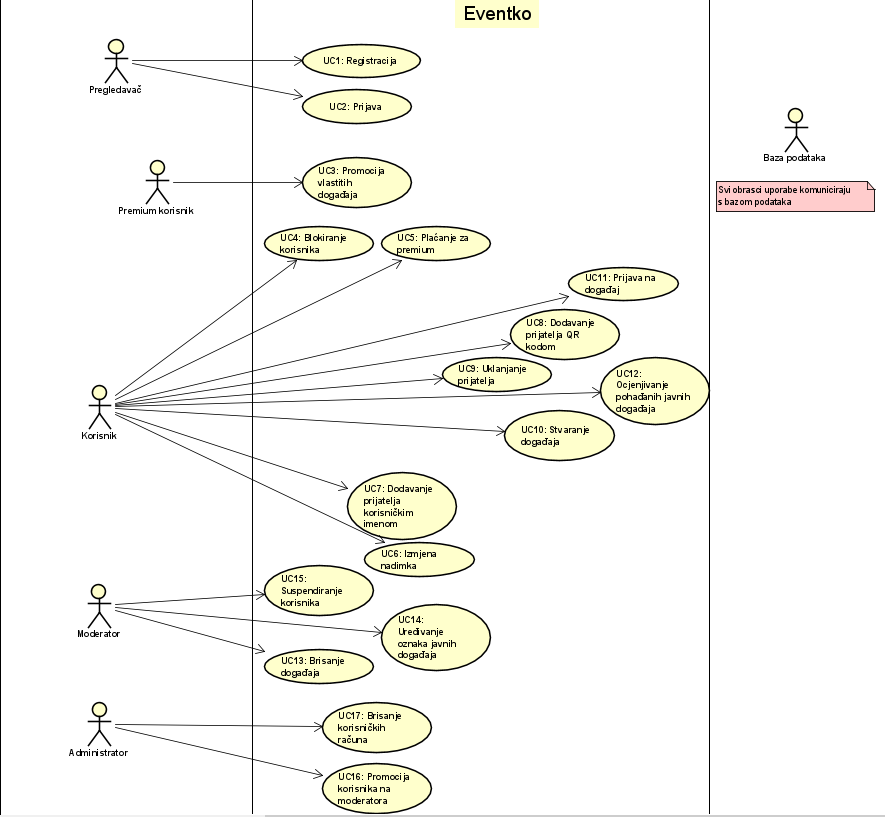
\includegraphics[width=\textwidth]{slike/UseCase.jpg}
						\caption{Dijagram obrazaca uporabe, funkcionalnosti različitih korisnika stranice}
					\end{figure}
														
				\eject		
				
			\subsection{Sekvencijski dijagrami}
				
				
				\noindent \textbf {Obrazac uporabe UC1 - Registracija}\\
				\indent {Korisnik šalje zahtjev za prikaz stranice za prijavu kako bi mogao odabrati gumb za registraciju. Korisnik onda šalje zahtjev za prikaz stranice za registraciju. Upisuje podatke potrebne za izradu računa koje Web aplikacija šalje bazi podataka koja radi profil. Baza vraća potvrdu nakon izrađenog profila i korisnik je vraćen na prikaz stranice za prijavu.   } \\

				\begin{figure}[h]
					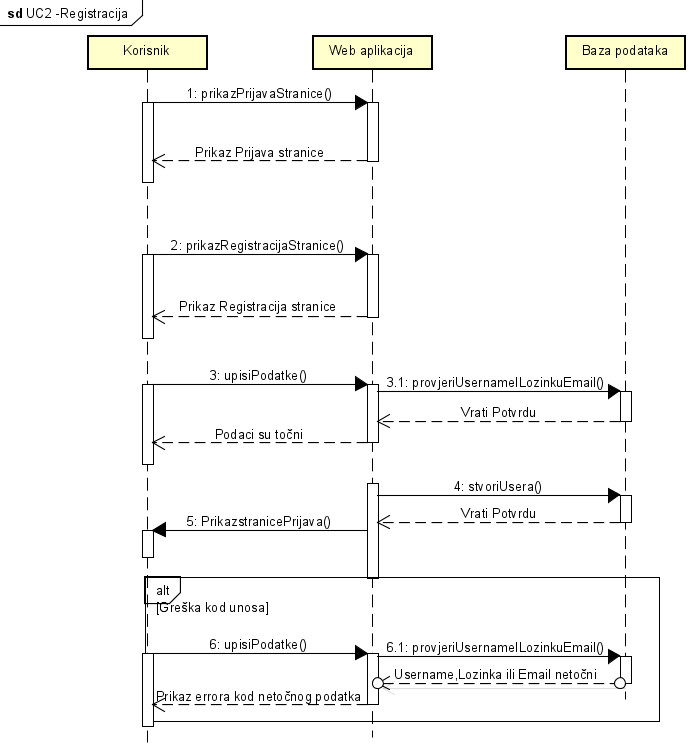
\includegraphics[width=\textwidth]{slike/Registracija.png}
					\caption{Sekvencijski dijagram za UC1}
				\end{figure}
						
			    \noindent {Ukoliko je došlo do greške pri upisu podataka, korisnik ostaje na stranici prijave i pojavljuje mu se error uz podatak koji je kriv. Moguće greške pri unosa podataka mogu se desiti ako za korisničko ime koristimo znakove koji nisu u engleskoj abecedi,brojeve 0-9, "\_" ili ako je kraće od 2 znaka. Greška se može desiti ako za nadimak ako sadrži manje od 2 ili više od 25 znakova. Email mora biti u formatu npr. ime@domena.hr. Lozinka mora sadržavati barem 4 znaka.}\\ \\
				
				
				\noindent \textbf {Obrazac uporabe UC2 - Prijava}\\
				\indent {Korisnik šalje zahtjev za prikaz stranice za prijavu nakon kojeg upisuje potrebne podatke. Web aplikacija šalje podatke bazi podataka koja dohvaća korisnike i traži zadanog korisnika prema imenu profila. Baza podataka vraća profil korisnika nakon kojeg je korisniku prikazana početna stranica. Ukoliko dođe do greške korisnik ostaje na stranici Prijava te mu je prikazan error poruka. Greška se može desiti ako koristimo korisničko ime i lozinku koji nisu povezani jedno uz drugo ili ne postoje. }\\
				
				\begin{figure}[h]
					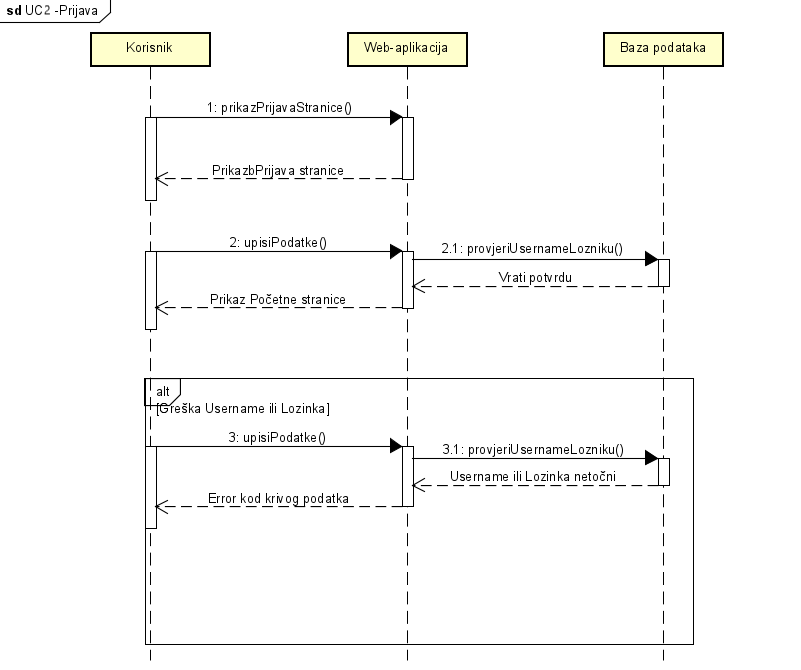
\includegraphics[width=\textwidth]{slike/Prijava.png}
					\caption{Sekvencijski dijagram za UC2}
				\end{figure}
				
				\eject
	
		\section{Ostali zahtjevi}
		 
			 \begin{packed_item}
			 \item  Sustav treba omogućiti rad više korisnika u stvarnom vremenu
			 \item Izvršavanje dijela programa u kojem se pristupa bazi podataka ne smije trajati duže od nekoliko sekundi
			 \item Sustav treba biti implementiran kao web aplikacija koristeći objektno-orijentirane jezike
			 \item Neispravno korištenje korisničkog sučelja ne smije narušiti funkcionalnost i rad sustava
			 \item Sustav treba biti jednostavan za korištenje, korisnici se moraju znati koristit sučeljem bez opširnih uputa
			 \item Nadogradnja sustava ne smije narušavati postojeće funkcionalnosti sustava
			 \item Veza s bazom podataka mora biti kvalitetno zaštićena, brza i otporna na vanjske greške
			 \end{packed_item}
	